
\section{GoF Design Pattern}

\begin{figure}[h]
    \centering
    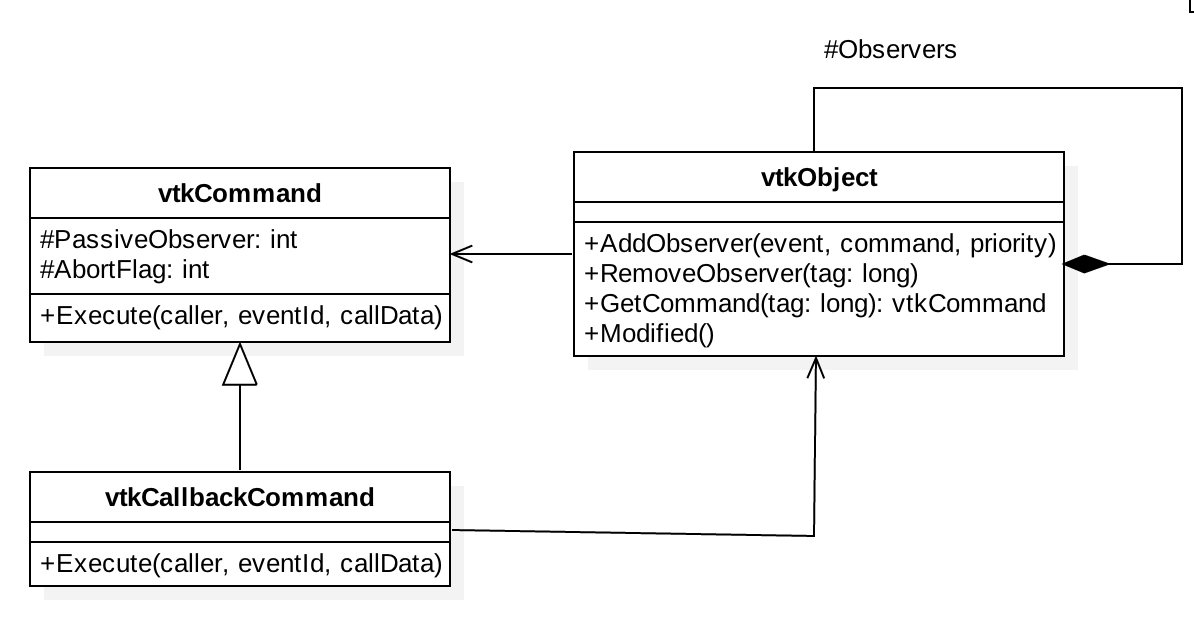
\includegraphics[width=8cm]{diagrams/design_pattern.png}
    \caption{Command/Observer design pattern}
    \label{fig::design::pattern}
\end{figure}

\begin{definition}
The command pattern is a behavioural design pattern in which an object is used to encapsulate all information needed to perform an action or trigger an event at a later time.
\end{definition}

\begin{definition}
The observer pattern is a behavioural design pattern in which an object, called the subject, maintains a list of its dependants, called observers, and notifies them automatically of any state changes, usually by calling one of their methods.
\end{definition}

VTK uses events and commands to allow users to interact with data and user interface. The toolkit response with appropriate commands to every event published by the lower components, creating a system based on two design patterns, Observer and Command. The user interface widgets use the Observer pattern to emit events and activate commands in other components.  

\subsection{Classes \& Interfaces}

VTK implements a combination between the command and observer design patterns using two primary classes \code{vtkObject} with controls the observer side of the problem, and \code{vtkCommand} with is an abstractisation of a concrete command such as \code{vtkCallbackCommand} \cite{git}.

As a language, C++ does not support stand-alone interfaces, like Java. The project uses abstract classes to represent interfaces for concrete components. The design decision behind \code{vtkObject} reflects the same design patterns used in Java's Object class.


\subsection{Roles \& Responsibilities}

The class \code{vtkObject} is the base class for most objects in the visualisation toolkit and provides methods for tracking modification time, debugging, printing, and event callbacks \cite{git}. The \code{vtkObject} also performs reference counting: objects that are reference counted exist as long as another object uses them. Once the last reference to a reference counted object is removed, the object will spontaneously destruct. 

The \code{vtkObject} represents the subject in observer design pattern; its able to add observers and notify them when the client is sending a command \code{vtkCommand}. Since \code{vtkObject} can also be notified using the method \code{Modified()}  \cite{git}, one can create a composition of \code{vtkObject} objects using its register/unregister observer features.

The observer/command design pattern is implemented by \code{vtkCommand}. In this design pattern, any instance of \code{vtkObject} can be "observed" for any events it might invoke. Observers of events are added with the \code{AddObserver()} method found in \code{vtkObject}.  

Event processing can be organised in priority lists, so it is possible to truncate the processing of a particular event by setting the \code{AbortFlag} variable. The priority is set using the \code{AddObserver()} method. By default the priority is 0, events of the same priority are processed in last-in-first-processed order  \cite{git}. When an instance of \code{vtkObject} invokes an event, it also passes an optional void pointer to a \code{callData}. 

For function callbacks, VTK uses \code{vtkCallbackCommand}, which can be used for function execution using the command/observer design pattern in VTK.

\subsection{Consequences}

\begin{consequences}
The combination of observer and command design pattern improves the routes of communication between the upper and lower level components.
\end{consequences}

\begin{consequences}
The observer pattern comes as a requirement since the toolkit uses widgets such as sliders in their user interface; those user interface components must notify other objects to change their state.
\end{consequences}
